\pagebreak
\section{Gauss Seidel [25\%]}
Consider the successively over-relaxed, left-to-right Gauss-Seidel iterative smoother applied to a standard, second-order, central-difference discretization of the 1D Poisson equation $(-u_{xx}=f)$ on $x\in [0,1]$ with homogeneous Dirichlet boundary conditions.  The grid is uniform and contains $N$ intervals.

\begin{enumerate}[label=\alph*., start = 1]
    \item Write  an  expression  for  the  iteration  matrix, $\doubleunderline{S}$,  for  this  smoother,  using  the  decomposition $\doubleunderline{A}=\doubleunderline{L}+\doubleunderline{D}+\doubleunderline{U}$,  where $\doubleunderline{A}\underline{u}=\underline{f}$ is the discretized system,  as in the notes.  Note that $\omega$ is a \underline{successive} over-relaxation factor, applied immediately on each node update.
    

    \vspace{-0.25in}
    \begin{gather*}
        \shortintertext{Since I will be implementing a second-order central-difference discretization of 1D Poisson's equation with homogeneous Dirichlet boundary conditions. The expression $\doubleunderline{A}\underline{u} = \underline{f}$}
        \underbrace{\begin{bmatrix}
            1 & 0 & 0 & 0 & \cdots & 0 & 0\\
           -1 & 2 & 1 & 0 & \cdots & 0 & 0\\
           0 & -1 & 2 & -1 & \cdots & 0 & 0\\
           0 & 0 & \ddots & \ddots & \ddots & 0 & 0\\
           \vdots & \vdots &  & \ddots & \ddots & \ddots &  \\
           0 & 0 & \cdots & 0 & -1 & 2 & -1\\
           0 & 0 & \cdots & 0 & 0 & 0 & 1
        \end{bmatrix}}_{\doubleunderline{A}} \underbrace{\begin{bmatrix}
            u_1\\ u_2\\ u_3\\ \vdots\\ \vdots\\ u_n\\ u_{n+1} \end{bmatrix}}_{\underline{u}}
            = \underbrace{\begin{bmatrix} 0\\ h^2f_2\\ h^2f_3\\ \vdots\\ \vdots\\ h^2f_n\\ 0 \end{bmatrix}}_{\underline{f}}\\
        \shortintertext{Re-writing $\doubleunderline{A}$ in terms of $\doubleunderline{L},\ \doubleunderline{D},\ \doubleunderline{U}$ gives,}
        \doubleunderline{L} = \begin{bmatrix}
            0 & 0 & 0 &  \cdots & 0\\
           -1 & 0 & 0 &  \cdots & 0\\
            0 & \ddots & 0  & 0 & 0\\
            0 & \cdots & -1 & 0 & 0\\
            0 & \cdots &  0 & 0 & 0
        \end{bmatrix},\quad \doubleunderline{D} = \begin{bmatrix}
            1 & 0 & 0 &  \cdots & 0\\
            0 & 2 & 0 &  \cdots & 0\\
            0 & 0 & \ddots  & \cdots & 0\\
            0 & \cdots & 0 & 2 & 0\\
            0 & \cdots & 0 & 0 & 1
        \end{bmatrix},\quad  \doubleunderline{U} = \begin{bmatrix}
            0 & -1 & 0 & \cdots & 0\\
            0 & 0 & \ddots & \cdots & 0\\
            0 & 0 & 0  & -1 & 0\\
            0 & \cdots & 0 & 0 & -1\\
            0 & \cdots & 0 & 0 & 0
        \end{bmatrix}\\
        \shortintertext{The smoothing iteration matrix is then given by,}
        \doubleunderline{S} = -\left(\doubleunderline{D} + \doubleunderline{L}\right)^{-1}\doubleunderline{U}
        \shortintertext{Doing so and creating a general expression for the matrix I get that $\doubleunderline{S}$ can be expressed to be,}
        \boxed{\doubleunderline{S} = \begin{bmatrix}
            0 & 0 & 0 & 0 & \cdots & \cdots & 0 & 0\\
            0 & 0 & \frac{1}{2} & 0 & \cdots & \cdots & 0 & 0\\
            0 & 0 & \frac{1}{4} & \frac{1}{2} & \ddots & \cdots & 0 & 0\\
            0 & 0 & \frac{1}{8} & \frac{1}{4} & \ddots & \ddots & 0 & 0\\
            0 & 0 & \vdots & \ddots & \ddots & \ddots & \ddots & 0\\
            0 & 0 & \frac{1}{2^{n-1}} & \cdots & \ddots & \ddots & \ddots & 0\\
            0 & 0 & \frac{1}{2^{n}} & \frac{1}{2^{n-1}} & \cdots & \frac{1}{8} & \frac{1}{4} & \frac{1}{2}\\
            0 & 0 & \cdots & \cdots & 0 & 0 & 0 & 0
        \end{bmatrix}}
    \end{gather*}

    \begin{fminipage}{0.9\linewidth}
        \textbf{Looking to the matrix above, it takes the form that the first two columns are completely zero and that the first/last rows are fully zero as well. Then along the lower matrix it follows a pattern of decreasing by factors of two from the value of the index above it. Meaning the values decrease in $\bf \frac{1}{2},\ \frac{1}{2^2},\ \frac{1}{2^3},\ \frac{1}{2^4}, \ldots, \frac{1}{2^{n-1}},\ \frac{1}{2^n}$ along the rows of the matrix along the diagonal.}
    \end{fminipage}

    \pagebreak
    \item In the complex number plane, plot the eigenvalues of the iteration matrix, $\doubleunderline{S}$, for this smoother,using $N= 32$ and an over-relaxation factor of $\omega = 1.5$.
    
    Plotting the eigenvalues of the iteration matrix by the formula,
    \begin{equation*}
        \lambda(\doubleunderline{S}_\omega) = \omega\lambda(\doubleunderline{S}) + (1 - \omega)
    \end{equation*}
    Gives the plot shown below in Figure \ref{fig:q3b},
    \begin{figure}[h]
        \centering
        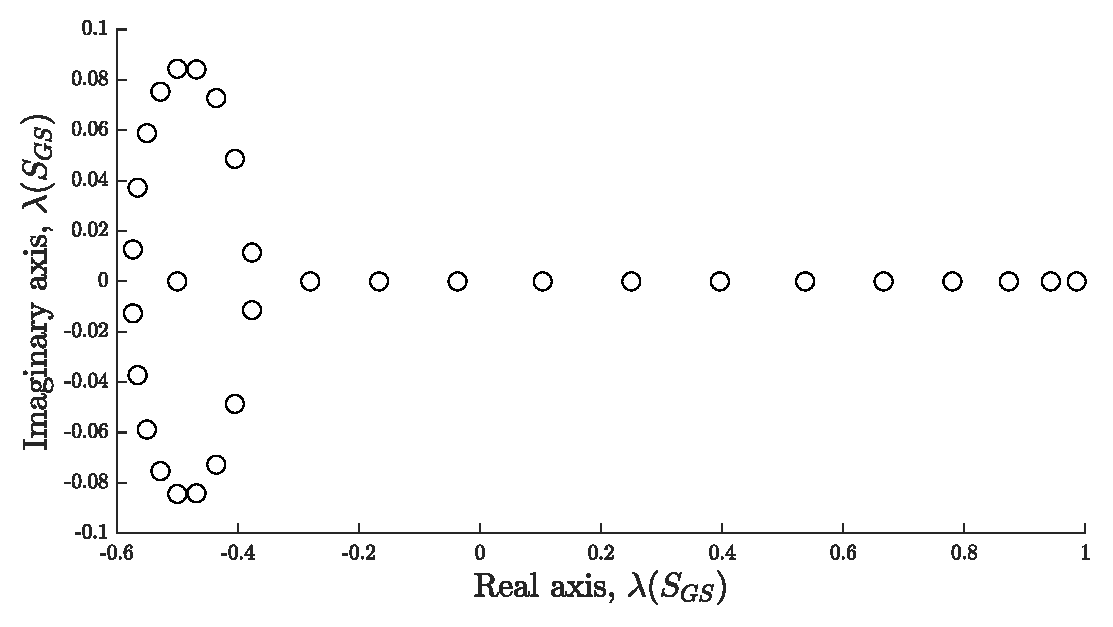
\includegraphics[width = 0.6\linewidth]{q3/q3_eigens.eps}
        \caption{Eigenvalues in the complex number plane.}
        \label{fig:q3b}
    \end{figure}

    
    \item Make a plot of the magnitude of the largest magnitude eigenvalue of $\doubleunderline{S}$ versus $\omega$, and identify the optimal over-relaxation factor. Use $N= 32$.
    
    \begin{figure}[h]
        \centering
        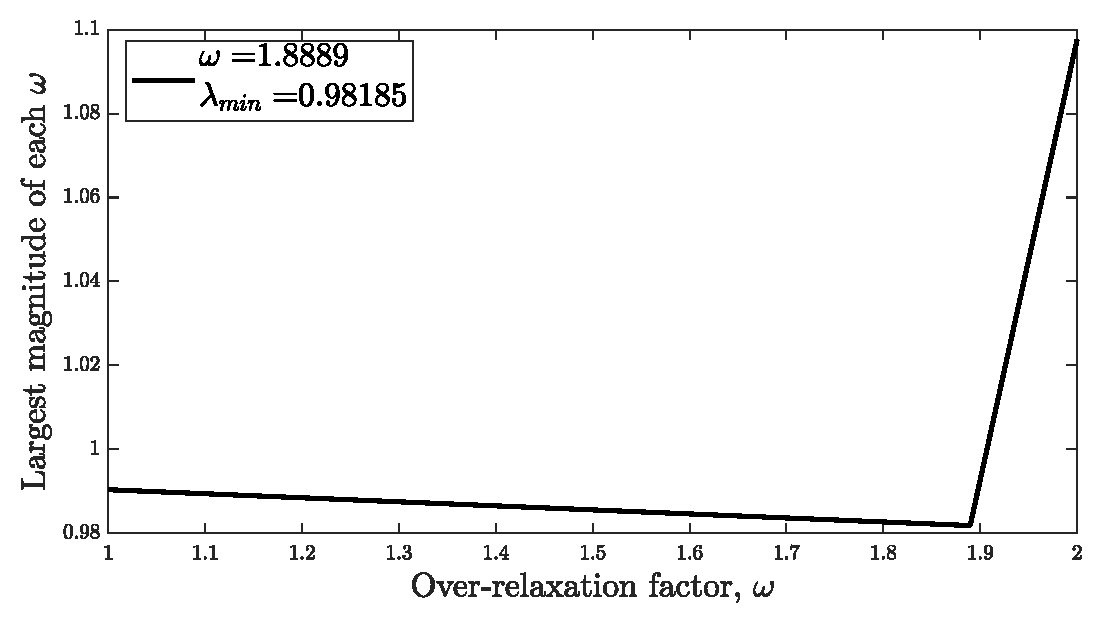
\includegraphics[width = 0.6\linewidth]{q3/q3_omegas.eps}
        \caption{Determining the optimal over-relaxation factor.}
        \label{fig:q3-over_relaxation}
    \end{figure}

    \begin{fminipage}{0.9\linewidth}
        \textbf{Looking above to Figure \ref{fig:q3-over_relaxation}, the optimal over-relaxation value occurs when the magnitude of the eigenvalues reach a minimum. This is because we need $\bf \lambda(\doubleunderline{S}) < 1$ for convergence and further from 1 for fast convergence. This minimum value can be found on the Figure to be $\bf \lambda_{min} = 0.98185$, at this minimum amplification factor the over-relaxation factor is found to be an optimal of $\bf \omega = 1.8889$. Any value of $\bf \omega$ greater than this value will risk deteriorating the convergence rates. Matlab code can be found attached at the end of my assignment.}
    \end{fminipage}
\end{enumerate}